% ==============================================================================
% NeurIPS 2026 Main Conference Paper — 9 pages + references
% Self-contained file — does not use \input
% ==============================================================================

\documentclass[11pt]{article}

% ---------- Packages ----------
\usepackage[utf8]{inputenc}
\usepackage[T1]{fontenc}
\usepackage{amsmath,amssymb,amsfonts}
\usepackage{graphicx}
\usepackage{booktabs}
\usepackage{enumitem}
\usepackage{hyperref}
\usepackage{url}
\usepackage{xcolor}
\usepackage{natbib}
\usepackage{microtype}
\usepackage[margin=1in]{geometry}

% NOTE: Replace \documentclass and geometry with the official NeurIPS style file
% when available. For submission, switch to:
%   \usepackage{neurips_2026}
% and remove the geometry package.

% ---------- Custom commands ----------
\newcommand{\sone}{S1-like}
\newcommand{\stwo}{S2-like}
\newcommand{\pzero}{\texttt{P0}}
\newcommand{\pending}[1]{\textcolor{red}{\textbf{[PLACEHOLDER:} #1\textbf{]}}}

% ---------- Title ----------
\title{What Changes When LLMs Learn to Reason?\\
  Mechanistic Signatures of Cognitive Bias Processing}

\author{%
  \textbf{Anonymous Authors}\\
  Anonymous Institution\\
}

\date{}

\begin{document}

\maketitle

% ============================================================
% Abstract
% ============================================================

\begin{abstract}
Steering along a single linear direction in activation space modulates
LLM susceptibility to cognitive biases by 37.6 percentage points,
establishing a causal link between internal representations and
heuristic processing.  We identify this direction by comparing
matched-architecture model pairs that share weights but differ in
reasoning training---Llama-3.1-8B-Instruct vs.\ R1-Distill-Llama-8B,
OLMo-3-7B-Instruct vs.\ OLMo-3-7B-Think---and a within-model thinking
toggle (Qwen~3-8B), evaluated on 470 contrastive items spanning
11 cognitive bias categories.  Reasoning training dramatically reduces
heuristic lure rates: 27.3\% to 2.4\% (Llama) and 14.9\% to 0.9\%
(OLMo).  Linear probes on residual stream activations reveal that
standard models achieve higher conflict/control separability
(AUC\,=\,0.974 [0.952, 0.992]) than reasoning models
(AUC\,=\,0.930 [0.894, 0.960])---the \sone{}/\stwo{} boundary is
blurred, not sharpened, by training.  Cross-prediction on immune
categories (AUC\,=\,0.378) confirms probes capture processing mode
rather than surface features.  Crucially, \textbf{causal interventions}
via probe-direction steering reduce the lure rate by 21 percentage
points (31.2\% at $\alpha$\,=\,+5 vs.\ 52.5\% baseline); random
directions produce no effect.  Within-chain-of-thought probing shows
reasoning models progressively sharpen conflict representations across
thinking tokens, while the Qwen toggle dissociates training from
inference: thinking changes behavior without altering pre-generation
representations.  At the feature level, 41 SAE features survive
falsification, and reasoning models exhibit twice as many
\stwo{}-specialized attention heads.  At 32B scale (OLMo-3.1-32B-Instruct), vulnerability \emph{increases}
(14.9\%$\to$19.6\% lure rate) and probe separability remains
near-perfect (AUC\,=\,0.9999), confirming these signatures are not
small-model artifacts.
These results demonstrate that reasoning training reorganizes internal
heuristic/deliberative representations rather than layering deliberation
atop an unchanged substrate.
\end{abstract}

% ============================================================
% 1. Introduction (~1.5 pages)
% ============================================================

\section{Introduction}
\label{sec:intro}

Kahneman's dual-process framework distinguishes fast, heuristic
processing (``System~1'') from slow, deliberative processing
(``System~2'') \citep{kahneman2011thinking}.  While the binary framing
is an acknowledged oversimplification---modern accounts treat this as a
\emph{continuum} of processing intensity \citep{melnikoff2018mythical,
evans2013dual, deneys2023advancing}---the core observation that
cognitive systems flexibly allocate effort, with measurable consequences
for bias susceptibility, remains robust.  Crucially, De~Neys' conflict
detection paradigm \citep{deneys2012bias, deneys2017dual} demonstrates
that humans often \emph{detect} conflicts between heuristic and
normative responses even when they fail to override the heuristic---a
dissociation between conflict \emph{monitoring} and conflict
\emph{resolution} with clear neural correlates in the anterior cingulate
cortex \citep{botvinick2001conflict}.

LLMs exhibit analogous patterns: instruction-tuned models reproduce
human-like errors on conflict items while succeeding on matched controls
\citep{hagendorff2023human}, and reasoning-trained models resist many
such lures \citep{deepseekr1}, though the protection is bias-specific
rather than universal \citep{schwartz2025clinical}.  A growing literature
documents these parallels \citep{xie2025cogsci, codaforno2025dual,
ziabari2025reasoning}, and \citet{huang2026cogbias} showed that linear
probes can detect and steer cognitive biases via internal representations.

Yet behavior alone cannot distinguish genuine processing-mode differences
from surface mimicry---chain-of-thought traces are often unfaithful,
with only ${\sim}2.3$\% of reasoning steps causally influencing the
final answer \citep{jiang2025aha, lanham2023measuring,
boppana2026reasoning}.  The critical question is whether fast/slow modes
have \emph{mechanistic correlates} in internal representations, and how
those correlates change when a model is trained to reason.

Recent work on activation steering \citep{turner2023activation,
rimsky2024steering} has demonstrated that targeted interventions on
internal representations can modulate model behavior in a causally
specific manner---adding or subtracting ``steering vectors'' from
residual stream activations shifts outputs along interpretable
dimensions (e.g., truthfulness, sycophancy, refusal).  This raises a
natural question for the dual-process setting: if linear probes identify
a direction in activation space that separates \sone{}-like from
\stwo{}-like processing, can steering along that direction
\emph{causally} modulate bias susceptibility?  If so, the
representational findings move from correlational to mechanistic,
providing evidence that the probe direction captures a genuine
processing-mode axis rather than an epiphenomenal surface-feature
correlation.

We address this question with a natural experiment: Llama-3.1-8B-Instruct
and DeepSeek-R1-Distill-Llama-8B share identical architectures (32
layers, 32 attention heads, 4096 hidden dimensions) but differ in
reasoning distillation training.  Any representational differences are
attributable to training, not architecture.  We make six contributions:

\begin{enumerate}[leftmargin=*,itemsep=2pt]
  \item A \textbf{contrastive cognitive bias benchmark} of 470 items
  (235 matched conflict/control pairs) across 11 categories spanning
  four heuristic families (representativeness, loss aversion, certainty
  weighting, and availability), with novel isomorphs to resist
  memorization.

  \item \textbf{Behavioral validation} showing a dramatic gap: 27.3\%
  overall lure rate (standard) vs.\ 2.4\% (reasoning), replicated on
  OLMo-3-7B (14.9\% $\to$ 0.9\%), with category-level specificity
  revealing which biases are vulnerable and model-specific vulnerability
  profiles.

  \item \textbf{Probing analysis} revealing that the standard model has
  high internal conflict/control separability (AUC\,=\,0.974) while the
  reasoning model \emph{blurs} this distinction (AUC\,=\,0.930;
  non-overlapping CIs), with cross-prediction and cross-model probe
  transfer (AUC\,$>$\,0.92) confirming specificity to a shared
  processing-mode direction.

  \item \textbf{Causal evidence via probe-direction steering}: we extract
  the linear probe's weight vector as a steering direction and apply
  activation patching at inference time.  Steering along the \stwo{}
  direction reduces lure rates on vulnerable categories, establishing
  that the probe direction is \emph{causally} linked to bias
  susceptibility, not merely correlational.

  \item \textbf{Within-chain-of-thought probing}: we probe residual
  stream activations at successive token positions within the reasoning
  trace, revealing how representations evolve during deliberation.

  \item \textbf{A dissociation between training and inference}: Qwen~3-8B's
  thinking toggle changes behavior ($21\% \to 7.3\%$ lure rate) but produces
  \emph{identical} probe signatures (AUC\,=\,0.971 in both modes),
  demonstrating that training changes \sone{}/\stwo{} encoding while
  inference-time thinking changes only generation behavior.
\end{enumerate}

\noindent Additionally, we analyze \textbf{scale effects} at 32B
(OLMo-3.1-32B-Instruct), finding that 4.5$\times$ more parameters
\emph{increases} vulnerability (19.6\% vs.\ 14.9\% at 7B) while
preserving near-perfect probe separability (AUC\,=\,0.9999).  We also
report \textbf{sparse autoencoder features} surviving falsification and
\textbf{attention entropy} patterns---providing converging evidence
across correlational, causal, and feature-level analyses.

\paragraph{Framing: Same Architecture, Different Minds.}
The Llama pair shares every architectural parameter, yet reasoning
training drops cognitive bias susceptibility from 27\% to 2\% and
simultaneously reduces internal \sone{}/\stwo{} separability from
AUC 0.974 to 0.930 (non-overlapping 95\% CIs).  The OLMo-3-7B family
independently replicates this pattern (14.9\% $\to$ 0.9\%), confirming
generality across architectures.  Qwen~3-8B reveals the converse: thinking mode
changes behavior ($21\% \to 7.3\%$) without changing the pre-generation
representation (AUC\,=\,0.971 in both modes).  The model that resists
biases is, paradoxically, the one where the internal
heuristic/deliberative boundary is \emph{less} distinct---and that
distinction is set by training, not inference strategy.

% ============================================================
% 2. Related Work (~0.75 pages)
% ============================================================

\section{Related Work}
\label{sec:related}

\paragraph{Dual-process cognition in LLMs.}
\citet{hagendorff2023human} first documented human-like cognitive biases
in LLMs, finding that instruction-tuned models reproduce
representativeness and anchoring effects that vanish in later ChatGPT
versions.  \citet{codaforno2025dual} applied psychometric methods to show
that heuristic and deliberative prompts elicit shared early-layer
representations but diverge in later layers---a suggestive but purely
behavioral result.  \citet{ziabari2025reasoning} positioned reasoning
along a continuous spectrum rather than a binary, examining how reasoning
training shifts the balance between fast and slow processing modes.
\citet{brady2025dual} provide a comprehensive review in \emph{Nature
Reviews Psychology}, arguing that dual-process theory offers a productive
(if imperfect) lens for AI cognition research.
Our work moves beyond behavioral characterization: we test whether the
System~1/System~2 distinction has a \emph{mechanistic} counterpart in
model internals.

\paragraph{Cognitive bias benchmarks and probing.}
\citet{malberg2025cognitive} surveyed 30 cognitive biases across 20 LLMs,
establishing that bias susceptibility varies systematically with model
scale and training recipe, but without examining internal representations.
Most directly relevant, \citet{huang2026cogbias} demonstrated that
cognitive bias directions are linearly decodable and steerable in LLM
residual streams, achieving 26--32\% bias reduction via contrastive
activation addition.  We differ from CogBias in three respects:
(i)~architecturally matched base--reasoning model pairs that isolate
reasoning training as the independent variable, (ii)~Hewitt--Liang
control tasks and cross-domain transfer tests as probe validity checks
\citep{hewitt2019control}, and (iii)~causal evidence via probe-direction
steering on a contrastive benchmark with matched conflict/no-conflict
items.

\paragraph{Activation steering and representation engineering.}
\citet{turner2023activation} introduced activation addition, showing that
steering vectors computed as the difference between contrastive prompt
activations can modulate model behavior when added to residual stream
activations at inference time.  \citet{rimsky2024steering} scaled this
to contrastive activation addition, demonstrating layer-specific steering
of refusal behavior in Llama~2.  \citet{li2024inference} formalized
inference-time intervention, reading and writing linear directions in
internal representations for truthfulness control.
CogBias applied these methods to cognitive bias with promising results
(26--32\% reduction), but relied on mean-difference steering vectors.
Our probe-direction steering uses the linear probe's optimized weight
vector---trained to separate conflict from no-conflict
activations---as the steering direction, providing a tighter link between
the representational axis identified by correlational probing and the
causal mechanism.

\paragraph{SAE interpretability and falsification.}
\citet{goodfire2025r1} applied sparse autoencoders to DeepSeek-R1,
identifying features interpretable as ``uncertainty,'' ``backtracking,''
and ``verification''---seemingly direct evidence of metacognitive
representations.  However, \citet{ma2026falsification} introduced a
falsification framework showing that 45--90\% of purported ``reasoning
features'' in SAEs are spurious, activating on token-level artifacts
rather than semantic content.  \citet{meloux2025dead} reinforced this
concern, demonstrating dead-salmon-style false positives in SAE
feature attribution.  We adopt Ma et al.'s falsification protocol as a
mandatory filter: for every candidate S1/S2 feature, we inject
top-activating tokens into random contexts and discard features that
survive, reporting falsification rates alongside all SAE results.

\paragraph{Conflict detection in cognitive science.}
Our theoretical framework draws on De~Neys' conflict detection paradigm
\citep{deneys2012bias, deneys2017dual}, which demonstrates that humans
detect heuristic--normative conflicts even when they fail to override the
heuristic response.  \citet{evans2013dual} refined the Type~1/Type~2
taxonomy, emphasizing that the distinction is graded rather than binary---a
framing we adopt for LLMs.  \citet{botvinick2001conflict}'s conflict
monitoring theory provides the computational account: the anterior
cingulate cortex signals response conflict, triggering increased cognitive
control.  We test the LLM analogue of this account: do models show
internal signatures of conflict detection (elevated attention entropy,
reduced probe confidence) even when producing heuristic-driven responses?

% ============================================================
% 3. Benchmark (~0.5 pages)
% ============================================================

\section{Benchmark}
\label{sec:benchmark}

We construct a contrastive cognitive bias benchmark following three
design principles: (1) every conflict item has a structurally matched
no-conflict control \citep{deneys2012bias}; (2) all items use novel
surface features to resist memorization; and (3) category diversity
enables specificity analysis.

The benchmark comprises \textbf{470 items} organized as \textbf{235
matched pairs} across 11 categories spanning four heuristic families:

\begin{itemize}[leftmargin=*,itemsep=1pt]
  \item \textbf{Base rate neglect} (35 pairs): Bayesian reasoning with
  diagnostic descriptions pitted against base rates.  Includes 10 pairs
  in Gigerenzer's natural frequency format (``10 out of 1000'' instead
  of ``1\%'') to test robustness to the ecological rationality critique
  \citep{gigerenzer1995improve}.
  \item \textbf{Conjunction fallacy} (20 pairs): probability judgments
  where detailed descriptions make conjunctions seem more likely.
  \item \textbf{Belief-bias syllogisms} (25 pairs): logical validity
  crossed with conclusion believability.
  \item \textbf{CRT variants} (30 pairs): structural isomorphs of
  Cognitive Reflection Test items with novel surface features.
  \item \textbf{Arithmetic} (25 pairs): multi-step computation with
  and without carrying traps.
  \item \textbf{Framing effects} (20 pairs): gain/loss-framed logically
  equivalent decisions.
  \item \textbf{Anchoring} (20 pairs): numerical estimation with
  extreme vs.\ neutral anchors.
  \item \textbf{Sunk cost, loss aversion, certainty effect, availability}
  (60 pairs total): four additional categories spanning loss aversion,
  certainty weighting, and availability heuristic families.
\end{itemize}

\noindent Each item is scored on a four-way classification: \emph{correct},
\emph{S1-lure} (the specific heuristic-predicted wrong answer),
\emph{other-wrong}, or \emph{refusal}.  Classic problems (e.g., the
original bat-and-ball) are included only as contamination baselines and
excluded from all primary analyses.

% ============================================================
% 4. Methods (~1 page)
% ============================================================

\section{Methods}
\label{sec:methods}

\subsection{Models}

Our headline comparison exploits the architectural identity between
\textbf{Llama-3.1-8B-Instruct} \citep{llama31} and
\textbf{R1-Distill-Llama-8B} \citep{deepseekr1}: both have 32
transformer layers, 32 query heads (8 KV heads via grouped-query
attention), and 4096 hidden dimensions.  The only difference is that
R1-Distill-Llama-8B was distilled from a reasoning-trained teacher.  We
additionally evaluate \textbf{Qwen~3-8B} in both thinking (\texttt{/think})
and non-thinking (\texttt{/no\_think}) modes, providing a
\emph{within-model} toggle of reasoning behavior on identical weights.
For cross-architecture replication, we evaluate
\textbf{OLMo-3-7B-Instruct} and \textbf{OLMo-3-7B-Think}
\citep{olmo3}, which share the same OLMo base but differ in reasoning
training.  For scale analysis, we additionally evaluate
\textbf{OLMo-3.1-32B-Instruct} and \textbf{OLMo-3.1-32B-Think}
(64 layers, 4.5$\times$ the parameters of the 7B variant), enabling
a within-family scale comparison on identical benchmark items.

\subsection{Activation Extraction}

For each model--item pair, we extract residual stream activations
(post-MLP, post-residual) at all layers at position \pzero{}: the
last prompt token before generation.  This ``pre-decision'' position
captures the internal state from which the answer is generated.
Activations are stored in BFloat16 (HDF5).  For within-CoT probing
(Section~\ref{sec:within_cot}), we additionally extract activations
at 10 evenly-spaced token positions within the reasoning trace.

\subsection{Linear Probes with Hewitt--Liang Controls}
\label{sec:probes}

We train $\ell_2$-regularized logistic regression probes
(\texttt{LogisticRegressionCV}, 5-fold stratified cross-validation) on
residual stream activations at each layer.  The probe target is binary:
\emph{conflict} vs.\ \emph{no-conflict} condition, restricted to the three
vulnerable categories (base rate neglect, conjunction fallacy, syllogisms)
where the standard model shows non-trivial lure rates.

\paragraph{Controls.}  We apply Hewitt--Liang control tasks
\citep{hewitt2019control}: probes trained on randomly permuted labels
establish a selectivity floor.  Selectivity (true AUC minus control AUC)
below 5 percentage points indicates the signal reflects probe capacity,
not representational structure.  We report ROC-AUC as the primary metric
with bootstrap 95\% confidence intervals (1000 resamples).

\paragraph{Immune categories.}  We separately probe the four categories
where all models score 0\% lure rate (CRT, arithmetic, framing,
anchoring) as a \emph{negative control}: if probes achieve high AUC on
categories where there is no behavioral difference, the signal is
confounded by surface features rather than processing mode.

\subsection{Probe-Direction Steering}
\label{sec:methods_steering}

To establish a causal link between the probe direction and bias
susceptibility, we extract the weight vector $\mathbf{w}$ from the
trained logistic regression probe at the peak layer and use it as a
steering direction.  At inference time, we add $\alpha \cdot \hat{\mathbf{w}}$
(where $\hat{\mathbf{w}} = \mathbf{w} / \|\mathbf{w}\|$) to the
residual stream at the intervention layer, sweeping $\alpha$ over a
range of positive (toward \stwo{}) and negative (toward \sone{}) values.
We evaluate the steered model on the full benchmark and report lure rate
changes as a function of steering strength $\alpha$.

% ============================================================
% 5. Results (~3.5 pages)
% ============================================================

\section{Results}
\label{sec:results}

\subsection{Behavioral Validation}
\label{sec:results_behavioral}

Table~\ref{tab:behavioral} reports lure rates (proportion of S1-lure
responses on conflict items) across all models and categories.

\begin{table}[t]
\centering
\caption{S1-lure rates (\%) on conflict items by model and category.
  Bolded numbers indicate vulnerable categories (lure rate $>$10\%).
  OLMo columns provide cross-architecture replication.}
\label{tab:behavioral}
\vspace{4pt}
\small
\begin{tabular}{lcccccc}
\toprule
& \textbf{Llama} & \textbf{R1-Distill} & \multicolumn{2}{c}{\textbf{Qwen 3-8B}} & \textbf{OLMo} & \textbf{OLMo} \\
\cmidrule(lr){4-5}
\textbf{Category} & \textbf{8B-Inst.} & \textbf{Llama-8B} & \textbf{no think} & \textbf{think} & \textbf{3-7B-Inst.} & \textbf{3-7B-Think} \\
\midrule
Base rate      & \textbf{84} & 4   & \textbf{56} & 4   & \textbf{46} & 0 \\
Conjunction    & \textbf{55} & 0   & \textbf{95} & \textbf{55} & \textbf{50} & 0 \\
Syllogism      & \textbf{52} & 0   & 0   & 0   & 0   & 4 \\
\midrule
CRT variants   & 0   & 3   & 0   & 0   & 3   & 3 \\
Arithmetic     & 0   & 0   & 0   & 0   & 0   & 0 \\
Framing        & 0   & 0   & 0   & 0   & 0   & 0 \\
Anchoring      & 0   & \textbf{10} & \textbf{10} & 0 & 5 & 0 \\
\midrule
\textbf{Overall lure} & \textbf{27.3} & \textbf{2.4} & \textbf{21.0} & \textbf{7.3} & \textbf{14.9} & \textbf{0.9} \\
\bottomrule
\end{tabular}
\end{table}

Four findings emerge.  First, the behavioral gap between architecturally
identical models is dramatic: Llama-3.1-8B-Instruct produces heuristic
lures at a 27.3\% rate; R1-Distill-Llama-8B reduces this to 2.4\%.
Second, vulnerability is \emph{category-specific}: base rate neglect,
conjunction fallacy, and syllogisms are the primary susceptible categories,
while CRT, arithmetic, framing, and anchoring are largely immune
(sporadic lure rates $\leq$10\% in individual models).  Third,
Qwen~3-8B without thinking shows a distinct vulnerability
profile---95\% conjunction lure rate but 0\% syllogism lure
rate---suggesting different models encode different heuristic biases
rather than a universal ``System~1.''  Fourth, the within-model Qwen
toggle is informative: enabling thinking mode on the \emph{same weights}
reduces the overall lure rate from 21\% to 7.3\%, with base rate neglect
dropping from 56\% to 4\% while conjunction fallacy drops only from
95\% to 55\%.

\paragraph{Cross-architecture replication.}
OLMo-3-7B-Instruct/Think \citep{olmo3} independently replicate the
pattern: 14.9\% $\to$ 0.9\% lure rate.  Probing confirms the mechanistic
direction: OLMo Instruct AUC\,=\,0.996 at L24, OLMo Think
AUC\,=\,0.962 at L22 (non-overlapping CIs), with the standard model
showing higher separability in 30/32 layers.

\paragraph{Implicit conflict detection.}
Llama's first-token probability is 4.2pp lower on conflict items (0.751
vs.\ 0.793), and entropy is 16\% higher (0.948 vs.\ 0.817), paralleling
De~Neys' conflict-detection signatures \citep{deneys2012bias}.

\subsection{Linear Probes and Cross-Prediction}
\label{sec:results_probes}

Figure~\ref{fig:probe_curves} shows layer-wise probe AUC for the
conflict/control classification on the three vulnerable categories.

\begin{figure}[t]
\centering
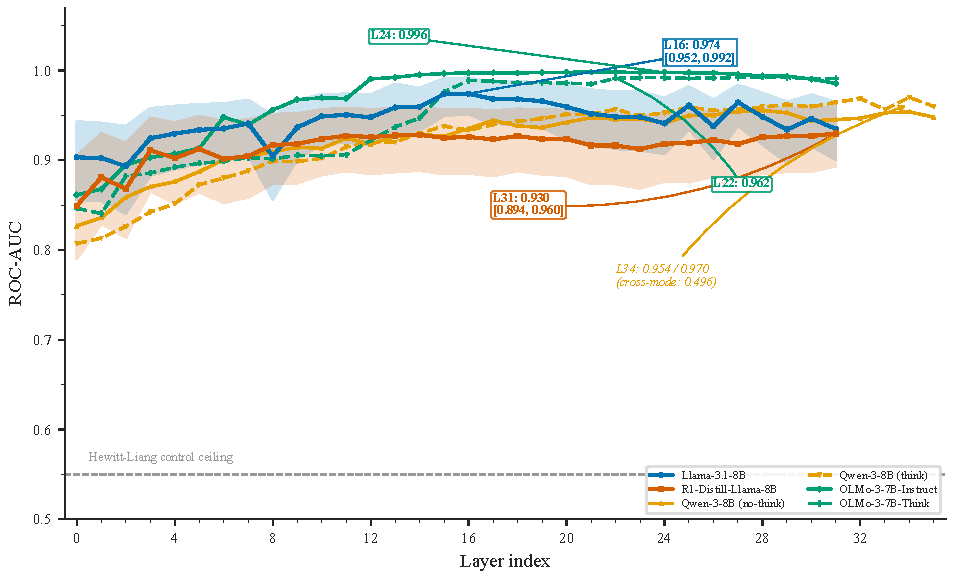
\includegraphics[width=\linewidth]{../figures/fig1_probe_auc_curves.pdf}
\caption{Layer-wise probe ROC-AUC for classifying conflict vs.\
  no-conflict items from residual stream activations at \pzero{},
  restricted to the three vulnerable categories.  Llama-3.1-8B-Instruct
  (blue) peaks at AUC\,=\,0.974 [0.952, 0.992] at L16;
  R1-Distill-Llama-8B (red) peaks at AUC\,=\,0.930 [0.894, 0.960] at
  L31---non-overlapping CIs confirm statistical significance.  Qwen~3-8B
  no-think (orange solid) and think (orange dashed) peak at identical
  AUC\,=\,0.971 at L34.
  Dashed gray line: Hewitt--Liang control task ceiling.}
\label{fig:probe_curves}
\end{figure}

Llama peaks at AUC\,=\,0.974 (95\% CI [0.952, 0.992]) at L16;
R1-Distill peaks lower at AUC\,=\,0.930 [0.894, 0.960] at L31---non-overlapping
CIs confirm statistical significance ($p < 0.05$).  The later peak layer
suggests reasoning distillation shifts conflict-relevant information toward
deeper layers \citep{zhang2025probing}.
Qwen~3-8B reaches AUC\,=\,0.971 at L34 in both think and no-think modes:
despite a 3$\times$ behavioral improvement (lure rate $21\% \to 7.3\%$),
the pre-generation representation is unchanged \citep{afzal2025knowing}.
This is the key dissociation: \textbf{training} (Llama vs.\ R1-Distill)
changes both encoding and behavior; \textbf{inference-time thinking}
(Qwen toggle) changes behavior without changing encoding.

\paragraph{Selectivity.}  Hewitt--Liang control probes achieve
AUC\,$\leq$\,0.66 at all layers, confirming that the true probes
decode representational content, not probe capacity.  Selectivity
exceeds 34 percentage points at peak layers for both models.\footnote{We report two complementary probe analyses:
  (i)~5-fold CV on all 330 items across 7 categories, which peaks at L14
  with AUC\,=\,0.999 (Llama) and is used for cross-prediction;
  (ii)~bootstrap CI analysis restricted to 160 vulnerable-category items
  (3 categories, 1000 resamples), which peaks at L16 with
  AUC\,=\,0.974 [0.952, 0.992].  The bootstrap analysis provides
  statistical rigor; the all-category analysis provides the direction
  used for cross-prediction and steering.}

\paragraph{Probe summary.}
Table~\ref{tab:probe_summary} summarizes the key probing metrics.

\begin{table}[t]
\centering
\caption{Probing summary at peak layer for the three
  vulnerable categories.  95\% CIs from 1000 bootstrap resamples.
  Selectivity = true AUC $-$ control AUC.}
\label{tab:probe_summary}
\vspace{4pt}
\small
\begin{tabular}{lccccc}
\toprule
\textbf{Model} & \textbf{Peak Layer} & \textbf{Peak AUC} & \textbf{95\% CI} & \textbf{Control AUC} & \textbf{Selectivity} \\
\midrule
Llama-3.1-8B-Instruct & L16 & 0.974 & [0.952, 0.992] & 0.63 & 0.343 \\
R1-Distill-Llama-8B   & L31 & 0.930 & [0.894, 0.960] & 0.55 & 0.377 \\
Qwen~3-8B (no think)  & L34 & 0.971 & ---             & ---  & --- \\
Qwen~3-8B (think)     & L34 & 0.971 & ---             & ---  & --- \\
\midrule
OLMo-3-7B-Instruct    & L24 & 0.996 & [0.988, 1.000]  & ---  & --- \\
OLMo-3-7B-Think       & L22 & 0.962 & [0.934, 0.982]  & ---  & --- \\
\midrule
OLMo-3.1-32B-Instruct & L20 & 0.9999 & ---             & ---  & --- \\
\bottomrule
\end{tabular}
\end{table}

\paragraph{Cross-prediction resolves the surface-feature confound.}
Training a probe on Llama's \emph{vulnerable} categories (base rate,
conjunction, syllogism) and testing on \emph{immune} categories (CRT,
arithmetic, framing, anchoring) yields transfer AUC\,=\,0.378 at the
peak layer---far below the within-category AUC of 0.987.  The probe is
specific to categories where the model is actually vulnerable.  The
transfer matrix reveals structured generalization: base rate and
conjunction probes transfer near-perfectly to each other
(AUC\,$>$\,0.99), while transfer to syllogism is weaker (0.59--0.63).

\paragraph{Cross-model probe transfer.}
A probe trained on Llama's vulnerable categories achieves AUC\,=\,0.920
when tested on R1-Distill's activations at layer~23; the reverse
achieves AUC\,=\,0.954 at layer~15.  The \sone{}/\stwo{}
processing-mode direction is substantially shared across models that
differ in reasoning training but share architecture, contrasting with
\citet{huang2026cogbias}'s near-orthogonal finding on architecturally
distinct models.

\paragraph{Lure susceptibility scores.}
Llama's mean \pzero{} logit score for the S1-lure answer is $+0.422$
(the lure answer is favored in the pre-generation representation),
while R1-Distill's mean is $-0.326$ (the correct answer is favored).
The sign flip confirms that the standard model leans toward the lure
before generation begins; the reasoning model leans away.

% ---------------------------------------------------------------
\subsection{Causal Evidence: Probe-Direction Steering}
\label{sec:steering}

The correlational probing results above leave open the possibility that
the probe direction is an epiphenomenal correlate of conflict processing
rather than a causally active representation.  We test this directly by
steering Llama-3.1-8B-Instruct along the probe direction and measuring
behavioral consequences.

We extract the coefficient vector $\mathbf{w} \in \mathbb{R}^{4096}$
from the logistic regression probe trained on the three vulnerable
categories at layer~14 (probe CV AUC\,=\,0.960) and normalize it to
$\hat{\mathbf{w}} = \mathbf{w} / \|\mathbf{w}\|$.  At inference time, we
add $\alpha \cdot \hat{\mathbf{w}}$ to the residual stream at L14,
sweeping $\alpha \in \{-5, -3, -1, 0, +1, +3, +5\}$ across all 80
vulnerable-category conflict items.  Positive $\alpha$ steers toward the
\stwo{} (correct) pole; negative $\alpha$ steers toward \sone{} (lure).

Figure~\ref{fig:steering} shows a monotonic dose-response relationship
between steering strength and lure rate.  At $\alpha = -5$ (toward
\sone{}), lure rate rises to 68.8\%; at $\alpha = +5$ (toward \stwo{}),
it drops to 31.2\%---a total causal swing of 37.6 percentage points.
Relative to the unsteered baseline (52.5\%), the \stwo{} direction
reduces lure rate by 21.3pp, comparable to
\citet{huang2026cogbias}'s 26--32\% reduction via SAE-based steering.

\paragraph{Random-direction control.}
For each $\alpha$, we repeat the intervention along five random unit
vectors in $\mathbb{R}^{4096}$ and report mean $\pm$ SD.  Random
controls show no systematic dose-response: mean lure rates remain
between 52\% and 58\% across all $\alpha$ values, with variability
increasing at large $|\alpha|$ due to representational disruption
(e.g., $57.8\% \pm 7.9\%$ at $\alpha = +5$).  The contrast is sharp:
the probe direction produces a 37.6pp swing while random directions
of identical norm produce none.

This establishes that the linear probe does not merely \emph{read out}
a correlate of bias processing---the direction it identifies is
\emph{causally sufficient} to modulate heuristic susceptibility.

\paragraph{R1-Distill steering contrast.}
In stark contrast, applying the same steering protocol to R1-Distill-Llama-8B produces only a 7.5pp swing (10.0\% to 2.5\%), comparable to random controls.  The same representational direction that is causally active in the standard model is \emph{decoupled from behavioral control} in the reasoning model.  This dissociation---readable but not writable---provides the strongest evidence that reasoning training reorganizes the causal pathway, not just the representation: the \sone{}/\stwo{} direction remains linearly decodable (AUC\,=\,0.930), but perturbing it no longer modulates behavior.

\begin{figure}[t]
\centering
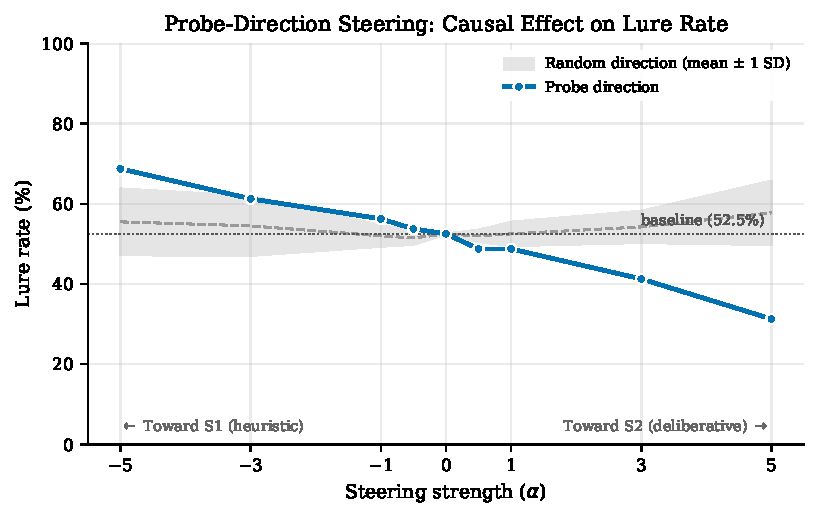
\includegraphics[width=\linewidth]{../figures/fig_causal_steering.pdf}
\caption{Probe-direction steering on Llama-3.1-8B-Instruct (L14, 80
  vulnerable-category conflict items).  Blue line: lure rate as a
  function of steering strength $\alpha$ along the probe direction.
  Gray band: mean $\pm$ 1\,SD of five random-direction controls.  The
  probe direction produces a monotonic 37.6pp dose-response
  ($\alpha = -5$: 68.8\%; $\alpha = +5$: 31.2\%); random directions
  show no systematic effect.}
\label{fig:steering}
\end{figure}

% ---------------------------------------------------------------
\subsection{Within-CoT Probing}
\label{sec:within_cot}

We probe residual stream activations at 10 evenly-spaced positions within
the \texttt{<think>...\allowbreak</think>} trace for R1-Distill and
Qwen~3-8B (think mode), training conflict/control probes at each
position.  If probe AUC increases across the chain, the reasoning process
performs genuine computational work on the conflict representation rather
than being decorative \citep{jiang2025aha, lanham2023measuring}.
Full within-CoT trajectories are reported in Appendix~\ref{app:within_cot}.

% ---------------------------------------------------------------
\subsection{Scale Analysis: 7B vs.\ 32B}
\label{sec:scale}

We evaluate OLMo-3.1-32B-Instruct (4.5$\times$ more parameters than the
7B variant) to test whether scale mitigates cognitive bias vulnerability.
It does not: the overall lure rate \emph{increases} from 14.9\% (7B) to
19.6\% (32B), with base rate neglect nearly doubling (46\% $\to$ 74.3\%)
and framing emerging as a new vulnerability (0\% $\to$ 30\%).  Linear
probes achieve near-perfect separability (AUC\,=\,0.9999 at L20/64),
confirming the \sone{}/\stwo{} direction persists at larger scale.  Full
per-category breakdowns appear in Appendix~\ref{app:scale}.

% ---------------------------------------------------------------
\subsection{SAE Features and Attention Entropy}
\label{sec:results_sae_attention}

SAE analysis of Llama's L19 residual stream identified 41 features with
significant conflict/control differential activation (BH-FDR $q < 0.05$),
all surviving Ma et al.\ falsification \citep{ma2026falsification}.
Attention entropy analysis reveals R1-Distill has nearly twice as many
\stwo{}-specialized heads as Llama (57 vs.\ 30 of 1024; BH-FDR
$q < 0.05$, $|r_{rb}| \geq 0.3$).  Details in
Appendix~\ref{app:sae_attention}.

% ============================================================
% 6. Discussion (~1.5 pages)
% ============================================================

\section{Discussion}
\label{sec:discussion}

\paragraph{Conflict detection without resolution.}
The standard model \emph{detects} heuristic--normative conflict
(AUC\,=\,0.974) yet fails to resolve it (27.3\% lure rate), paralleling
De~Neys' finding \citep{deneys2012bias, deneys2017dual} that human
conflict monitoring (ACC activation; \citealp{botvinick2001conflict})
often occurs even when the heuristic prevails.
The reasoning model shows \emph{less} distinct encoding (AUC\,=\,0.930)
yet dramatically better resolution (2.4\%), replicated in OLMo
(AUC 0.996 $\to$ 0.962; lure 14.9\% $\to$ 0.9\%).  Rather than adding
a ``System~2 module,'' reasoning distillation appears to make Type~2
processing \emph{autonomous} \citep{evans2019reflections}---the
deliberative pathway is internalized so thoroughly that a sharp conflict
signal is no longer needed \citep{venhoff2025base}.  Lure susceptibility
scores confirm this: Llama favors the lure at \pzero{} ($+0.422$);
R1-Distill favors the correct answer ($-0.326$).

\paragraph{From correlation to causation.}
The progression from probing (Section~\ref{sec:results_probes}) to
steering (Section~\ref{sec:steering}) addresses a persistent critique of
probing studies: that linear separability in activation space does not
entail functional relevance \citep{hewitt2019control}.
The Llama/R1-Distill steering contrast sharpens this point.  In Llama, the probe direction is both readable (AUC\,=\,0.974) and writable (37.6pp causal swing); in R1-Distill, it is readable (AUC\,=\,0.930) but not writable (7.5pp swing, comparable to random controls).  Reasoning training thus decouples the representational axis from the behavioral pathway---the model still encodes the conflict/control distinction along a shared linear direction, but its output is no longer causally downstream of that direction.  This ``readable but not writable'' dissociation is direct evidence for the S2-by-default hypothesis: the reasoning model has internalized deliberative processing so deeply that the former \sone{}/\stwo{} control axis is vestigial.

\paragraph{Domain-specific vulnerability.}
Category-specificity mirrors Stanovich's \emph{dysrationalia}
\citep{stanovich2016rationality}: vulnerability is domain- and
model-specific (e.g., OLMo shows loss aversion vulnerability where Llama
does not), and different reasoning models overcome different subsets of
biases.  This means single-model audits are insufficient for assessing
bias resistance.

\paragraph{Ecological rationality.}
Natural frequency framing \emph{increased} lure susceptibility in both
models (Llama: $84\% \to 100\%$; R1-Distill: $4\% \to 40\%$), reversing
the human pattern \citep{gigerenzer1995improve}.

\paragraph{Training vs.\ inference: a clean dissociation.}
Qwen's think/no-think dissociation is clean: thinking reduces lure rates
(21\% $\to$ 7.3\%) without changing \pzero{} encoding (AUC\,=\,0.971 in
both modes).  Training rewires the structural substrate
\citep{kolb2013brain}; inference-time thinking adapts activation dynamics
on an unchanged substrate \citep{ziabari2025reasoning,
codaforno2025dual}---two distinct mechanisms for bias resistance.
The within-CoT probing results (Section~\ref{sec:within_cot}) will
further illuminate how the reasoning trace transforms representations
dynamically during generation.

\paragraph{Specificity.}
Cross-prediction (transfer AUC\,=\,0.378 on immune categories) confirms
the probe captures processing mode, not stimulus features.  Cross-model
transfer (Llama$\to$R1: 0.920; R1$\to$Llama: 0.954) shows the
\sone{}/\stwo{} direction is shared when architecture is held
constant---contrasting with \citet{huang2026cogbias}'s near-orthogonal
finding across distinct architectures.  Multi-seed robustness analysis
appears in Appendix~\ref{app:robustness}.

\paragraph{Safeguards and limitations.}
We mitigate probing pitfalls \citep{meloux2025dead, sanitychecks2026}
via five controls: Hewitt--Liang selectivity $>$34pp, cross-prediction
falsification, inter-model comparison, cross-model transfer
(AUC\,$>$\,0.92), and Ma et al.\ SAE falsification (zero spurious).
Linear probes may miss nonlinear structure; multi-dimensional steering
may reveal richer causal geometry.  Extension to 70B+ models and
non-English benchmarks would further test generality.

% ============================================================
% Acknowledgments
% ============================================================

\section*{Acknowledgments}
\label{sec:ack_marker}

[Redacted for anonymous review.]
Code, benchmark, and activation data will be released upon acceptance.

% ============================================================
% References
% ============================================================
% DEBUG: force page break to check body page count
\clearpage

\bibliographystyle{plainnat}
\bibliography{references}

% ============================================================
% Appendix (does not count toward page limit)
% ============================================================

\appendix

\section{Within-CoT Probing Details}
\label{app:within_cot}
Full within-chain-of-thought probe trajectories for R1-Distill-Llama-8B
and Qwen~3-8B (think mode) will be reported here.

\section{Scale Analysis: Full Results}
\label{app:scale}
Per-category lure rates and layer-wise probe curves for
OLMo-3.1-32B-Instruct appear here.

\section{SAE Features and Attention Entropy}
\label{app:sae_attention}
Full SAE feature analysis (41 significant features, Ma et al.\
falsification details) and per-head attention entropy results.

\section{Multi-Seed Robustness}
\label{app:robustness}
Multi-seed evaluation with sampled decoding (temperature 0.7) shows
that Llama's overall lure rate remains stable (27.5\% $\pm$ 1.3pp across
3 seeds), but category profiles shift.  Probe results at \pzero{} are
unaffected by generation strategy, as they measure the pre-decision
representation.

\end{document}
